\documentclass{beamer} 

\usepackage[utf8]{inputenc}
\usepackage{graphicx}
\usepackage{multicol}
\usepackage{listings}


\begin{document}

\title{Uvod u funkcionalno programiranje}
\author{Stefan Nožinić (stefan@lugons.org)}

\frame{
\titlepage
}

\frame{
\frametitle{Uvod}
\begin{itemize}
  \item LISP 1950te
  \item Deklarativni stil 
  \item Imutabilnost 
  \item Thread-safeness 
\end{itemize}
}

\begin{frame}[fragile]
  \frametitle{Primer promene stanja u C}
  \begin{lstlisting}
#include <stdio.h>

int f( int* x ) 
{
  int res = (*x) + 1;
  (*x)++;
  return res;
}

int main() {
  int x = 5;
  printf("%d\n", f(&x));
  printf("%d\n", f(&x));
  return 0;
}
  \end{lstlisting}
\end{frame}

\frame{
\begin{itemize}
  \item Funkcija f povećava x za jedan i vraća x+1
  \item f menja stanje od x
  \item Ako ne vidimo definiciju funkcije f, ne znamo šta ona zapravo radi sa vrednostima ulaznih parametara!
  \item Da li uvek možemo da tvrdimo da je f(x) == f(x)?
\end{itemize}
}

\frame{
\frametitle{Prednosti nemenjanja stanja promenljivih}

\begin{itemize}
  \item Kompajler će ispisati grešku kada pokušamo promeniti stanje
  \item Svaka funkcija za iste ulazne parametre vraća istu povratnu vrednost
  \item Moguće lako paralelizovati program jer nema promene stanja promenljive 
\end{itemize}
}

\frame{
\frametitle{Data in - data out model} 
\begin{itemize}
  \item Primenjivo nezavisno od jezika
  \item Svaka funkcija vraća neku vrednost 
  \item Za isti ulaz, funkcija uvek vraća isti izlaz
  \item Funkcija ne zavisi od globalnog okruženja (globalne promenljive, IO, ...)
  \item Funkcija ne modifikuje sopstveni ulaz 
  \item Moguće primeniti i u OOP kodu - svaki setter vraća novi objekat 
  \item Primer: lista
\end{itemize}
}

\begin{frame}[fragile]
  \frametitle{Lista u C}
  \begin{lstlisting}
typedef struct ListElem_t
{
  int value;
  struct ListElem_t* next;
} ListElem;
  \end{lstlisting}
\end{frame}

\begin{frame}[fragile]
  \frametitle{Konstruktor elementa liste}
  \begin{lstlisting}

ListElem* create_element(int value, ListElem* next)
{
  ListElem* elem = (ListElem*) malloc(
    sizeof(ListElem)
  );
  elem->value = value;
  elem->next = next;
  return elem;
}

  \end{lstlisting}
\end{frame}


\begin{frame}[fragile]
  \frametitle{Lista struktura}
  \begin{lstlisting}

typedef struct
{
  ListElem* head;
} List;

  \end{lstlisting}
\end{frame}

\begin{frame}[fragile]
  \frametitle{Konstruktor liste}
  \begin{lstlisting}
List* create_list(ListElem* head)
{
  List* l = (List*) malloc(sizeof(List));
  l->head = head;
  return l;
}
  \end{lstlisting}
\end{frame}


\begin{frame}[fragile]
  \frametitle{Dodavanje elementa u listu}
  \begin{lstlisting}
List* push(List* l, int value)
{
  return create_list(create_element(
    value, l->head
  ));
}
  \end{lstlisting}
\end{frame}

\begin{frame}[fragile]
  \frametitle{Rep liste}
  \begin{lstlisting}
List* tail(List* l)
{
  return create_list(l->head->next);
}
  \end{lstlisting}
\end{frame}


\begin{frame}[fragile]
  \frametitle{print funkcija za ispis liste - zbog debug-a}
  \begin{lstlisting}
void print(List* l)
{
  if (l->head == NULL) printf("\n");
  else
  {
    printf("%d ", l->head->value);
    print(tail(l));
  }
}
  \end{lstlisting}
\end{frame}

\begin{frame}[fragile]
  \frametitle{main}
  \begin{lstlisting}
int main() {
  List *l = create_list(NULL);
  push(l, 5);
  print(l);
  List* l2 = push(l, 5);
  print(l2);
  
  print(tail(l2));
  print(push(l2, 10));
  return 0;
}
  \end{lstlisting}
\end{frame}

\frame{
\begin{itemize}
  \item Pure functional 
  \item Funkcije ne modifikuju parametre 
  \item Funkcije UVEK vraćaju rezultat
  \item Funkcija može primiti funkciju kao parametar
  \item Funkcija može vratiti funkciju kao rezultat
  \item Kompajlira se ali se može i interpretirati interaktivno
  \item ghc i ghci
  \item ".hs" ekstenzija se obično koristi za fajlove sa kodom
  \item Strogo tipovan - svaka vrednost mora imati svoj tip i jasno se zna šta je kog tipa tokom kompajliranja
\end{itemize}
}

\begin{frame}[fragile]
  \frametitle{Primer funkcije koja računa kvadrat izraza}
  \begin{lstlisting}
    sq :: Int -> Int
    sq x = x*x
  \end{lstlisting}
\end{frame}


\begin{frame}[fragile]
  \frametitle{Primer upotrebe alata ghci}
  \begin{lstlisting}
    ghci example.hs 
    >>> sq 5 
    25
    >>>
  \end{lstlisting}
\end{frame}


\begin{frame}[fragile]
  \frametitle{Primer funkcije koja računa zbir ulaznih parametara}
  \begin{lstlisting}
add :: Int -> Int -> Int 
add a b = a+b
  \end{lstlisting}
\end{frame}

\frame{
\begin{itemize}
  \item Funkcija u Haskell-u prima samo jedan parametar
  \item Funkcija `add` je funkcija koja prima jedan parametar i koja vraća funkciju koja prima drugi parametar i vraća zbir ta dva parametra
  \item inc = add 1 je funkcija koja vraća ulaz uvećan za jedan
\end{itemize}
}

\frame{
\begin{itemize}
  \item Jednostruko-povezane liste
  \item l = [1,2,3]
  \item head l 
  \item tail l 
  \item reverse l 
  \item last l 
  \item l = l1 ++ l2
  \item 5 : l
  \item range = [1..5]
  \item range = [1, 1.01..5]
\end{itemize}
}


\begin{frame}[fragile]
  \begin{lstlisting}
squares = [x*x | x <- [1..10]]

squaresDiv3 = [x*x | x <- [1..10], 
  x*x `mod` 3 == 0
]

unitcircle = 
  [(x,y) | 
    x <- [0, 0.01..10], 
    y <- [0,0.01..10], x*x + y*y < 1
  ]
  \end{lstlisting}
\end{frame}

\frame{
\frametitle{Pattern matching}
\begin{itemize}
  \item Fukciju je moguće definisati specifično za neke ulazne parametre
  \item Neka vrsta zamene za "if" tako da kod izgleda lepo
  \item Može se koristiti za "otpakivanje" podataka u složenim tipovima kao što je lista
\end{itemize}
}

\begin{frame}[fragile]
  \frametitle{Faktorijel - primer pattern matching-a} 
  \begin{lstlisting}
fact :: Int -> Int
fact 0 = 1
fact n = n * (fact (n-1))
  \end{lstlisting}
\end{frame}

\begin{frame}[fragile]
  \frametitle{Funkcija koja vraća jedinicu ako je bar jedan ulaz jednak nuli}
  \begin{lstlisting}
anyzero :: Int -> Int -> Int
anyzero 0 x = 1
anyzero x 0 = 1
anyzero x y = 0
  \end{lstlisting}
\end{frame}


\begin{frame}[fragile]
  \frametitle{Neke funkcije koje rade sa listama}
  \begin{lstlisting}

mymap :: (a -> b) -> [a] -> [b]
mymap _ [] = []
mymap f (x:xs) = (f x) : (mymap f xs)

myfilter :: (a -> Bool) -> [a] -> [a]
myfilter _ [] = [] 
myfilter f (x:xs) = 
  if (f x) then x : (myfilter f xs) 
  else myfilter f xs

  \end{lstlisting}
\end{frame}

\begin{frame}[fragile]
  \frametitle{Upotreba}
  \begin{lstlisting}
  *Main> mymap (+ 1) [1,2,3]
  [2,3,4]
  *Main> myfilter (\x -> x `mod` 2 == 0) [1,2,3,4,5,6]
  [2,4,6]

  \end{lstlisting}
\end{frame}
    

\begin{frame}
  \frametitle{fold}
  \begin{itemize}
    \item krenemo od funkcije sum pa ćemo da je generalizujemo
  \end{itemize}
\end{frame}

\begin{frame}[fragile]
  \frametitle{Obična suma brojeva}
  \begin{lstlisting}
sum :: [Int] -> Int
sum [] = 0
sum [x:xs] = x + (sum xs)
  \end{lstlisting}
\end{frame}


\begin{frame}[fragile]
  \frametitle{Obična suma brojeva - ali sada imamo drugačiji neutralni element!}
  \begin{lstlisting}
sum :: Int -> [Int] -> Int
sum z []  = z
sum z [x:xs] = x + (sum z xs )
  \end{lstlisting}
\end{frame}

\begin{frame}[fragile]
  \frametitle{Zamenimo + sa generalnom funkcijom f}
  \begin{lstlisting}
sum :: (Int -> Int -> Int) -> Int -> [Int] -> Int
sum f z []  = z
sum f z [x:xs] = f x  (sum f z xs )
  \end{lstlisting}
\end{frame}


\begin{frame}[fragile]
  \frametitle{E al sad nam ne treba više Int, sad može šta hoćemo!}
  \begin{lstlisting}
reduce :: (a -> b -> b) -> b -> [a] -> b
reduce f z []  = z
reduce f z [x:xs] = f x  (sum f z xs )
  \end{lstlisting}
\end{frame}



\begin{frame}
  \frametitle{Ilustracija fold-a}
  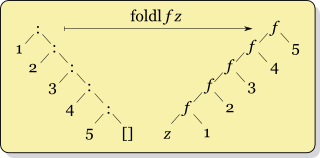
\includegraphics[width=\textwidth]{png/foldl.png}
\end{frame}

\begin{frame}
  \frametitle{Ilustracija desnog fold-a}
  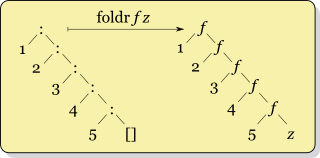
\includegraphics[width=\textwidth]{png/foldr.png}
\end{frame}

\begin{frame}[fragile]
  \frametitle{Upotreba}
  \begin{lstlisting}
*Main> reduce (+) 0 [1,2,3,4,5]
15
*Main> 
  \end{lstlisting}
\end{frame}

\begin{frame}[fragile]
  \frametitle{Funkcija koja vraća listu gde dva ista elementa nisu jedan do drugog} 
  \begin{lstlisting}

norepeat :: (Eq a) => [a] -> [a]
norepeat [] = [] 
norepeat (x:[]) = [x]
norepeat (x:y:xs) = if x == y 
then norepeat (x:xs) 
else x:(norepeat (y:xs))

  \end{lstlisting}
\end{frame}
    

\begin{frame}[fragile]
  \frametitle{Upotreba}
  \begin{lstlisting}

*Main> norepeat [1,1,2,5,5,6]
[1,2,5,6]
*Main> norepeat [1,1,2,5,5,6, 6]
[1,2,5,6]
*Main> norepeat [1,2,5,5,6, 6]
[1,2,5,6]
*Main> norepeat [1,2,5]
[1,2,5]
*Main>

  \end{lstlisting}
\end{frame}


\begin{frame}[fragile]
  \frametitle{Quick sort}
  \begin{lstlisting}
qsort :: [Int] -> [Int]
qsort [] = []
qsort l = 
  (qsort [x | x<-l, x < y]) 
  ++ [y] 
  ++ (qsort [x | x<-l, x>y]) where y = (head l)
  \end{lstlisting}
\end{frame}
    

\frame{
\frametitle{Tipovi podataka}
\begin{itemize}
  \item Definišu se tako što se navede ime tipa i njegovi konstruktori
  \item data NoviTip = konstruktor1 | konstruktor2 | ... 
  \item data Shape = Rectangle Int Int | Circle Int | Square Int 
\end{itemize}
}

\begin{frame}[fragile]
  \frametitle{Primer funkcije nad tipom}
  \begin{lstlisting}
data Shape = Circle Float | Rectangle Float Float 
area :: Shape -> Float 
area (Circle r) = r*r*3.14
area (Rectangle a b) = a*b
  \end{lstlisting}
\end{frame}
    
\begin{frame}[fragile]
  \frametitle{Binarno stablo}
  \begin{lstlisting}
data TreeNode = Node {
left :: Node,
right :: Node,
value :: Int
} | EmptyNode

tolist :: TreeNode -> [Int]
tolist EmptyNode = []
tolist n = let l = tolist $ left n
  r = tolist $ right n
  v = value n
  in l ++ [v] ++ r
  \end{lstlisting}
\end{frame}

\begin{frame}[fragile]
  \frametitle{Binarno stablo}
  \begin{lstlisting}
append :: TreeNode -> Int -> TreeNode
append EmptyNode x = Node EmptyNode EmptyNode x
append n x = let v = value n
  r = right n
  l = left n
  in if x < v 
  then Node (append l x) r v 
  else Node l (append r x) v

fromlist :: [Int] -> TreeNode -> TreeNode
fromlist [] n = n
fromlist l n = let x = head l
  in fromlist (tail l) (append n x)

bstsort :: [Int] -> [Int]
bstsort l = tolist (fromlist l EmptyNode)
  \end{lstlisting}
\end{frame}


\frame{
\frametitle{Monade}
\begin{itemize}
  \item Način da se promeni stanje 
  \item U realnom svetu, pojavljuje se potreba za moguč=ćnošću da se stanje može promeniti
  \item Primer: IO
  \item Monada uokviruje postojeći tip sa dodatnim informacijama koje se provlače kroz izračunavanje. 
  \item Potrebno implementirati:
  \begin{itemize}
    \item Tip podataka 
    \item return funkciju - a - > m a 
    \item bind funkciju - m a -> (a -> m a) -> m a
  \end{itemize}
  \item return ne utiče na izračunavanje 
  \item bind vezuje dva izračunavanja - poput kompozicije
\end{itemize}
}

\begin{frame}[fragile]
  \frametitle{Unit monada}
  \begin{lstlisting}

data Unit a = Unit a deriving (Show)

instance Monad Unit where 
return x = Unit x
(>>=) (Unit x) f = f x
  \end{lstlisting}
\end{frame}
  
\begin{frame}[fragile]
  \frametitle{Maybe monada}
  \begin{lstlisting}
data Maybe a = Just a | Nothing

instance Monad Maybe where 
return x = Just x
(>>=) (Nothing) _ = Nothing
(>>=) (Just x) f = f x
  \end{lstlisting}
\end{frame}

\begin{frame}[fragile]
  \frametitle{IO monada - hello world}
  \begin{lstlisting}
main :: IO ()
main = putStrLn "Hello world!" 

ghc hello.hs -o hello -dynamic 

  \end{lstlisting}
\end{frame}

  
\frame{
  \frametitle{WTF?????}
  \begin{itemize}
    \item IO monada je hak 
    \item IO moada je izlaz u realni svet 
    \item IO monada čuva redni broj tako da funkcije se ne optimizuju od strane kompajlera već se uvek izvršavaju!
  \end{itemize}
}

\begin{frame}[fragile]
  \frametitle{State}
  \begin{lstlisting}
data State s a = State (s -> (a,s))  

instance Monad (State s) where 
    return x = State $ \s -> (x,s)  
    (State h) >>= f = 
      State $ \s -> let (a, newState) = h s  
                  (State g) = f a  
                  in  g newState  

  \end{lstlisting}
\end{frame}

\begin{frame}
  \frametitle{Zaključak}
  \begin{itemize}
    \item Deklarativni stil
    \item Ne mora Haskell - principi primenljivi na druge jezike!
    \item Manje bagova 
    \item Lakše testirati softver
  \end{itemize}

  

\end{frame}

\end{document}
